% !TeX encoding = UTF-8
% !TeX spellcheck = en_GB
% !TeX root = ../D4.3a_User_Manual.tex
%
%
%
\section{Test Automation and Model Checking}\label{sec:Verification}
Test Automation and Model Checking for INTO-CPS is provided by the
RT-Tester RTT-MBT tool.
%
This section first describes installation and configuration of RT-Tester MBT
in Section \ref{section:rttester:installation}.
It then describes test automation in Section
\ref{sec:TestAuto} and model checking in Section
\ref{section:model:user-interface-integration}.
Note, that these features are explained in more detail in the deliverables
D5.2a \cite{INTOCPSD5.2a} and D5.3c \cite{INTOCPSD5.3c}, respectively.
Section \ref{sec:modeling.guidelines.TA.MC} describes modelling guidelines for model checking and model-based testing.
%
%
%
\subsection{Installation of RT-Tester RTT-MBT}\label{section:rttester:installation}

In order to use RTT-MBT, a number of software packages must be installed.
These software packages have been bundled into two installers:
\begin{itemize}
    \item \textbf{VSI tools dependencies bundle:}\\
    This bundle is required on the Windows
    platform and installs the following third party software:
    \begin{itemize}
        \item Python~2.7.
        \item GCC~4.9 compiler suite, used to compile FMUs.
    \end{itemize}
    \item \textbf{VSI tools -- VSI Test Tool Chain:}
    \begin{itemize}
        \item RT-Tester 6.0, a stripped version of the RT-Tester core test system that contains the necessary functionality for INTO-CPS.
        \item RT-Tester MBT 9.0, the model-based testing extension of RT-Tester.
        \item RTTUI 3.9, the RT-Tester graphical user interface.
        \item Utility scripts to run RTT-MBT.
        \item Examples for trying out RTT-MBT.
    \end{itemize}
\end{itemize}
%
%
%
These bundles can be downloaded via the download manager of the INTO-CPS Application.

\subsubsection{Setup of the RT-Tester User Interface}
When the RT-Tester User Interface (RTTUI) is first started, a few configuration
settings must be made.
%
%
%
\begin{itemize}
    \item User name and company name (\autoref{figure:rtt-mbt.config.user}).
    \item\label{item:vsi:config:bash} Location of Bash shell (\autoref{figure:rtt-mbt.config.bash}).
    This step can be safely skipped by clicking \emph{Next}.
    \item Path to Python~2.7 executable (\autoref{figure:rtt-mbt.config.python}):
    Click \emph{Detect} and then \emph{Installation Path} for auto-detection,
    or \emph{Browse} to select manually.
    \item Location of RT-Tester (\autoref{figure:rtt-mbt.config.rttester}):
    Click \emph{Browse} to select the directory of your RT-Tester installation.
    Note that if you did not specify the Bash shell location in step \ref{item:vsi:config:bash},
    the version number might not be detected properly.
\end{itemize}
%
%
%
\begin{figure}[ht]
    \begin{subfigure}{0.4\textwidth}
        \centerline{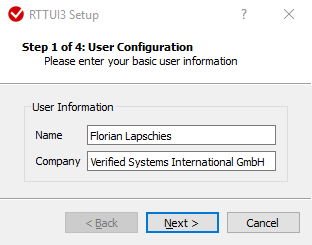
\includegraphics[scale=0.45]{figures/VSI-Configuration-User}}
        \caption{Configuring user.}
        \label{figure:rtt-mbt.config.user}
    \end{subfigure}
    \begin{subfigure}{0.6\textwidth}
        \centerline{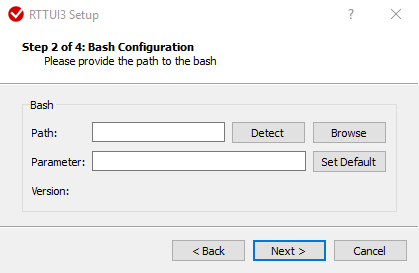
\includegraphics[scale=0.45]{figures/VSI-Configuration-Bash}}
        \caption{Configuring Bash.}
        \label{figure:rtt-mbt.config.bash}
    \end{subfigure}
    
    \begin{subfigure}{0.5\textwidth}
        \centerline{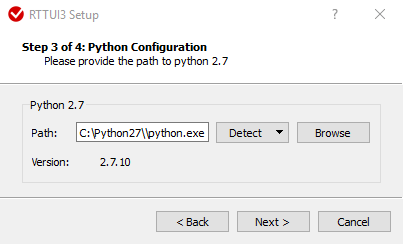
\includegraphics[scale=0.45]{figures/VSI-Configuration-Python}}
        \caption{Configuring Python.}
        \label{figure:rtt-mbt.config.python}
    \end{subfigure}
    \begin{subfigure}{0.5\textwidth}
        \centerline{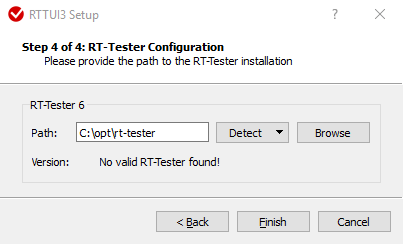
\includegraphics[scale=0.45]{figures/VSI-Configuration-Rttester}}
        \caption{Configuring RT-Tester.}
        \label{figure:rtt-mbt.config.rttester}
    \end{subfigure}
    \caption{RT-Tester GUI configuration.}
\end{figure}
%
%
%
\subsection{Test Automation}\label{sec:TestAuto}
Configuring and using a Test Project involves several activities.  These are:
%
%
%
\begin{itemize}
    \item Creating a test project.
    \item Defining tests.
    \item Compiling test driver FMUs.
    \item Setting up test runs.
    \item Running tests.
    \item Evaluating test results.
\end{itemize}
%
%
%
These activities can be performed either solely using the
RT-Tester graphical user interface,
or using a combination of the INTO-CPS Application and the RT-Tester GUI.
In this section we focus on describing the latter, since it supports the complete set of features necessary for test automation.
%
A more comprehensive description of the test automation workflow can
be found in Deliverable D5.2a \cite{INTOCPSD5.2a}.

In the INTO-CPS Application, test automation functionality can be found
below the main activity \emph{Test-Data-Generation} in the project browser.
%
Before using most of the test automation utilities,
the license management process has to be started.
To this end, right-click on \emph{Test-Data-Generation} and
select \emph{Start RT-Tester License Dongle}
(see Figure~\ref{figure:INTO-CPS-App:TDG:Start-License-Dongle}).
%
%
%
\begin{figure}[ht]
    \centerline{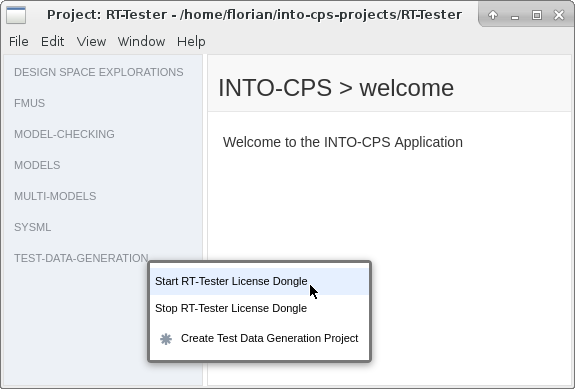
\includegraphics[width=0.8\textwidth]{figures/VSI-TDG_Start-License-Dongle}}
    \caption{Starting the license management process.}
    \label{figure:INTO-CPS-App:TDG:Start-License-Dongle}
\end{figure}
%
%
%

After developing the behavioural model in Modelio and
exporting it to an XMI file (see \cref{sec:SysML:BehaviouralModelling}), test automation projects can
be created from the INTO-CPS Application.
Such a project is then added as a sub-project within a containing
INTO-CPS Application project.
%
To create a project, do the following:
%
%
%
\begin{enumerate}
\item  Right-click on \emph{Test-Data-Generation}
in the project browser and select \emph{Create Test Data Generation Project} (see Figure~\ref{figure:INTO-CPS-App:Create-TDG-Project}).
%
\item  Specify a name for the project, select the XMI file containing the test model and press \emph{Create}, as shown in Figure \ref{figure:INTO-CPS-App:Create-TDG-Project-Dialog}.
\end{enumerate}
%
%
%
\begin{figure}[ht]
    \centerline{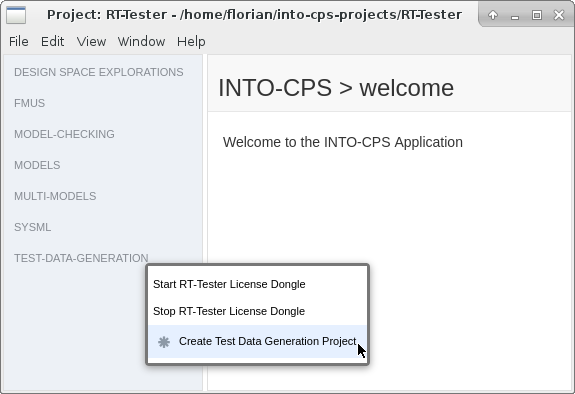
\includegraphics[width=0.8\textwidth]{figures/VSI-TDG_Create-TDG-Project}}
    \caption{Creating a test automation project.}
    \label{figure:INTO-CPS-App:Create-TDG-Project}
\end{figure}
%
%
%
\begin{figure}[ht]
    \centerline{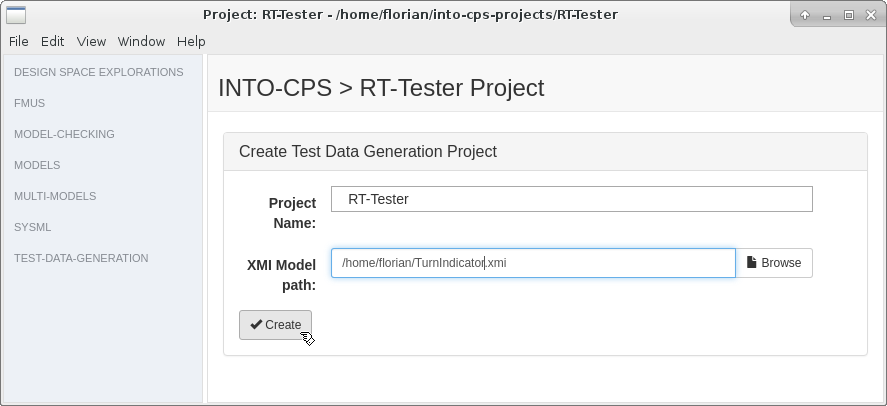
\includegraphics[width=\textwidth]{figures/VSI-TDG_Create-TDG-Project-Dialog}}
    \caption{Test automation project specifics.}
    \label{figure:INTO-CPS-App:Create-TDG-Project-Dialog}
\end{figure}
%
%
%
The newly created sub-project and its directory hierarchy is displayed in the
project browser.
The following two folders are of special significance:
%
%
%
\begin{itemize}
    \item \path{TestProcedures} contains symbolic test procedures where test objectives
    are specified in an abstract way, for example by specifying Linear Temporal Logic (LTL) formulas.
    \item 
    From these symbolic test procedures, concrete executable ({RT-Tester~6}) test procedures
    are generated, which then reside in the folder \path{RTT_TestProcedures}.
\end{itemize}

The specification of test objectives is done using the RT-Tester GUI.
The relevant files can be opened in the RT-Tester GUI directly from the
INTO-CPS Application by double-clicking them:
%
%
%
\begin{itemize}
    \item \path{conf/generation.mbtconf} allows you to specify the overall test objectives
      of the test procedure.
      Test objectives can be specified as LTL formulas, which must then be
      fulfilled during a test run.
      Test goals can also be specified by selecting structural elements from
      a tree representation of the test model and then choosing a coverage metric
      for that element. For example, the user might select a sub-component of
      the System Under Test (SUT) and specify that all Basic Control States (BCS) must be reached
      (see Figure \ref{figure:RTTUI:goals}),
      or that all transitions must be exercised (TR) in a test run.
    \item \path{conf/signalmap.csv} allows you to configure the input and output
      signals of the system under test (see Figure \ref{figure:RTTUI:signals}).
      This includes defining the admissible signal latencies for checking the SUT's outputs
      in a test run.
      This file also allows you to restrict the range of the signals in order to constrain
      these values during test data generation.
\end{itemize}
%
%
%
\begin{figure}[ht]
    \begin{center}
        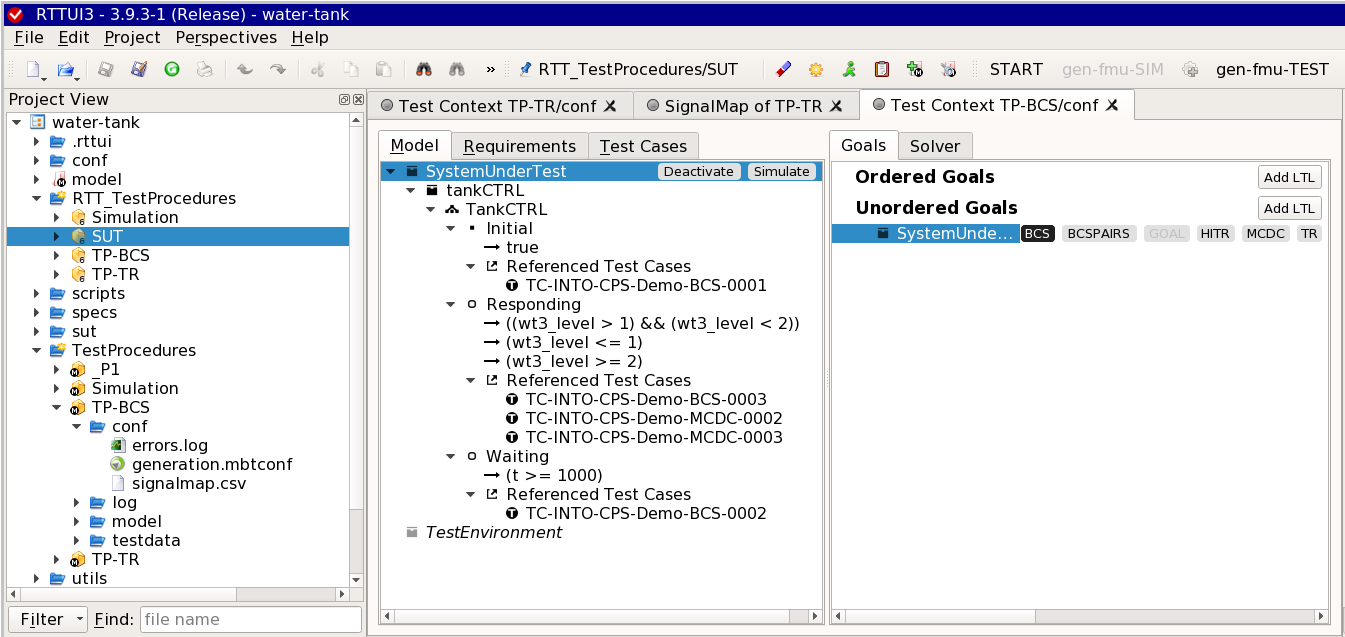
\includegraphics[width=1.0\textwidth]{figures/VSI-TDG_sc-rttui-goals-bcs} 
    \end{center}
    \caption{Configuring a test goal.}
    \label{figure:RTTUI:goals}
\end{figure}
%
%
%
\begin{figure}[ht]
    \begin{center}
        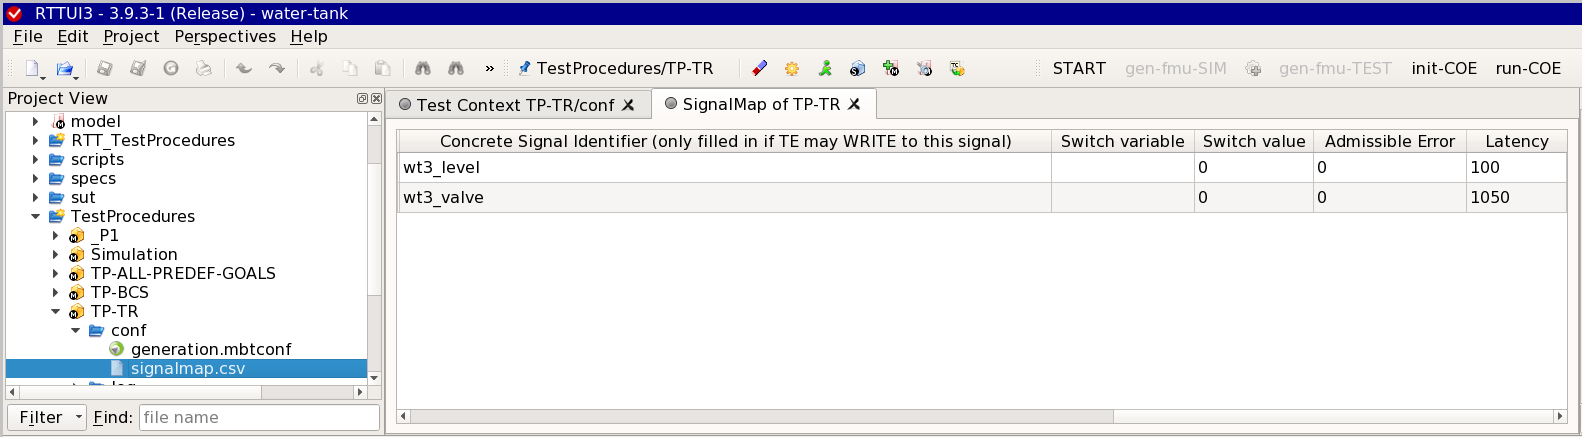
\includegraphics[width=1.0\textwidth]{figures/VSI-TDG_sc-mbt-configure-latency} 
    \end{center}
    \caption{Configuring signals.}
    \label{figure:RTTUI:signals}
\end{figure}
%
%
%
More details on the definition of tests can be found in Deliverable D5.2a \cite{INTOCPSD5.2a}.

After defining the test objectives, a concrete test case can be created by right-clicking on the symbolic test case under \emph{TestProcedures} and then
selecting \emph{Solve} (see Figure~\ref{figure:INTO-CPS-App:Solve}).
%
%
%
\begin{figure}[ht]
    \centerline{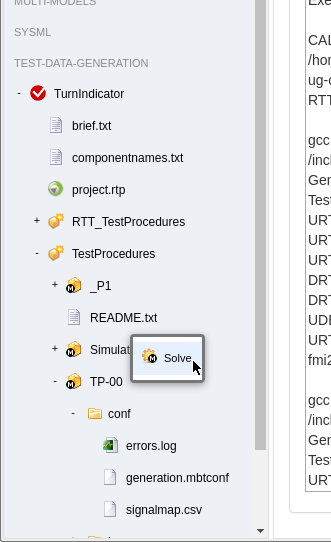
\includegraphics[width=0.4\textwidth]{figures/VSI-TDG_Solve}}
    \caption{Generating a concrete test procedure.}
    \label{figure:INTO-CPS-App:Solve}
\end{figure}
\clearpage
%
%
%
A solver component then computes the necessary timed inputs to realize the test
objectives. 
A concrete test procedure is generated that feeds a system under
test with these inputs and observes its outputs against expected results derived from the test model.
This test procedure will be placed in \path{RTT_TestProcedures} and has the same
name as the symbolic test procedure. Figure~\ref{figure:INTO-CPS-App:Solve-Progress}
shows how test generation progresses.
%
%
%
\begin{figure}[ht]
    \centerline{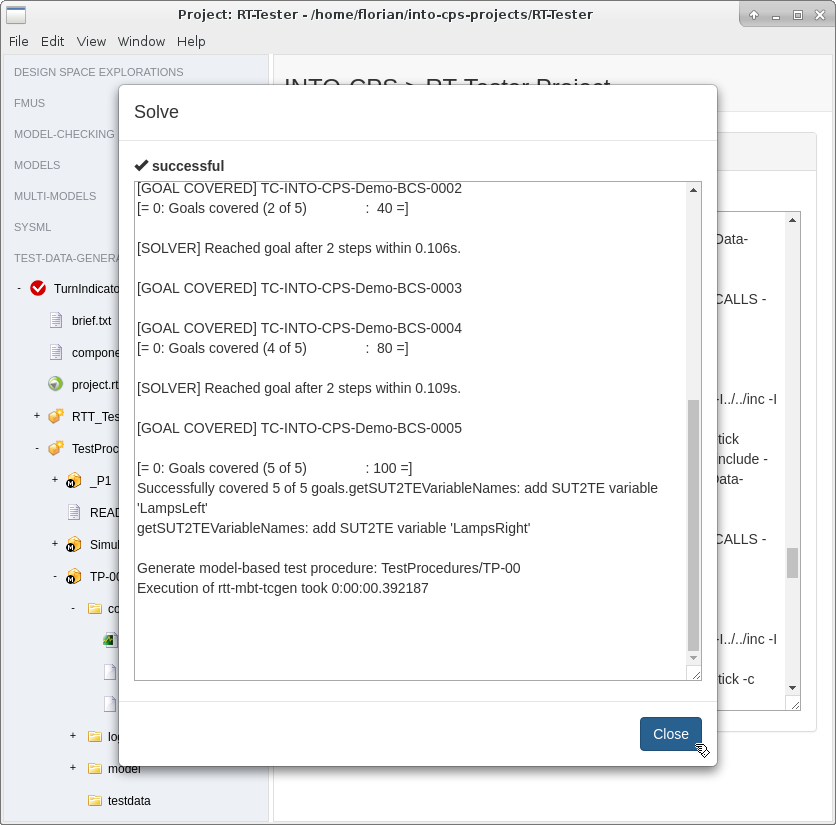
\includegraphics[scale=0.4]{figures/VSI-TDG_Solve-Progress}}
    \caption{Test data generation progress.}
    \label{figure:INTO-CPS-App:Solve-Progress}
\end{figure}
%
%
%

A generated test procedure can be cast into an FMU, which can then be
run in a co-simulation against the system under test.
To this end, right click on the concrete test procedure and select
\emph{Generate Test FMU} (see Figure~\ref{figure:INTO-CPS-App:Generate-Test-FMU}).
%
%
%
\begin{figure}[ht]
    \centerline{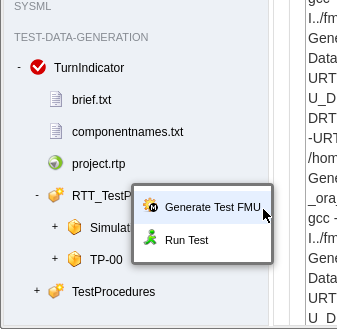
\includegraphics[width=0.4\textwidth]{figures/VSI-TDG_Generate-Test-FMU}}
    \caption{Generating a test FMU.}
    \label{figure:INTO-CPS-App:Generate-Test-FMU}
\end{figure}
%
%
%
In cases where a real and perhaps physical system under test is not available,
a simulation of the system under test can be generated from the behavioural model.
To generate such an FMU, right-click on \emph{Simulation} an select
\emph{Generate Simulation FMU} as depicted in 
Figure~\ref{figure:INTO-CPS-App:Generate-Simulation}.
%
%
%
\begin{figure}[ht]
    \centerline{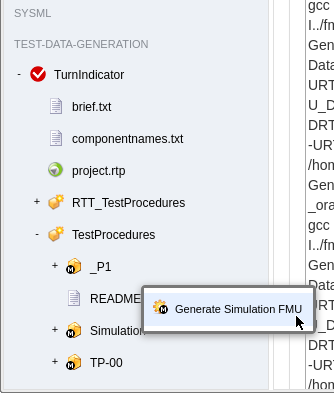
\includegraphics[width=0.4\textwidth]{figures/VSI-TDG_Generate-Simulation}}
    \caption{Generating a simulation FMU.}
    \label{figure:INTO-CPS-App:Generate-Simulation}
\end{figure}
%
%
%

In order to run a test, right-click on the test procedure and select
\emph{Run Test} (see Figure~\ref{figure:INTO-CPS-App:Run-Test}).
%
%
%
\begin{figure}[ht]
    \centerline{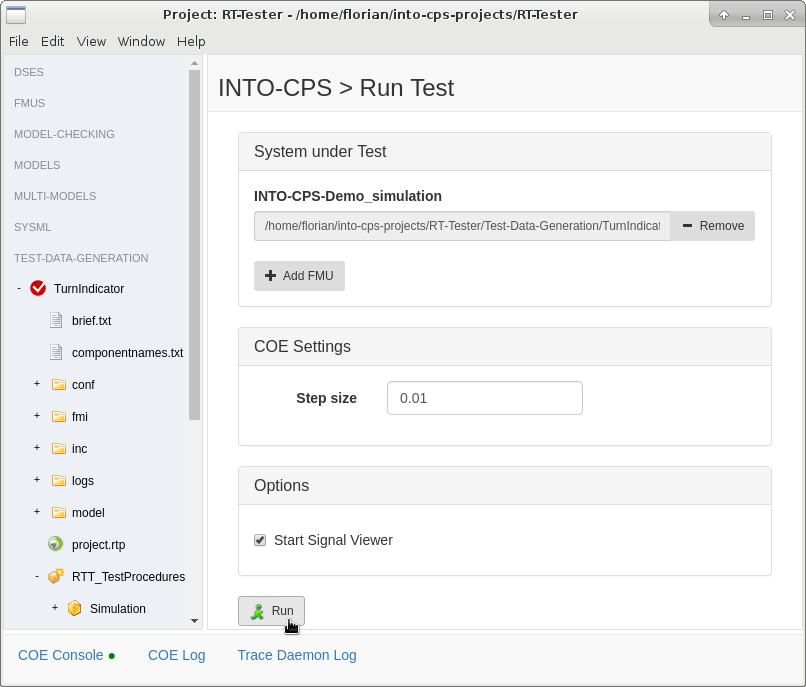
\includegraphics[width=0.6\textwidth]{figures/VSI-TDG_Run-Test}}
    \caption{Running a test.}
    \label{figure:INTO-CPS-App:Run-Test}
\end{figure}
%
%
%
Then, the FMUs that constitute the system under test must be added by pressing the
respective \emph{Add FMU} button.
When running a test, this list of FMUs is further augmented by an FMU representing
the test driver.
The connections between these FMUs are automatically derived by matching the
names of inputs and outputs.
The duration of the test is derived during test data generation
and does not need to be manually specified.
However, an appropriate step size must be set.
Finally, after making sure the COE is running, press \emph{Run} to start the test
(see Figure~\ref{figure:INTO-CPS-App:Run-Test-Dialog}).
%
%
%
\begin{figure}[ht]
    \centerline{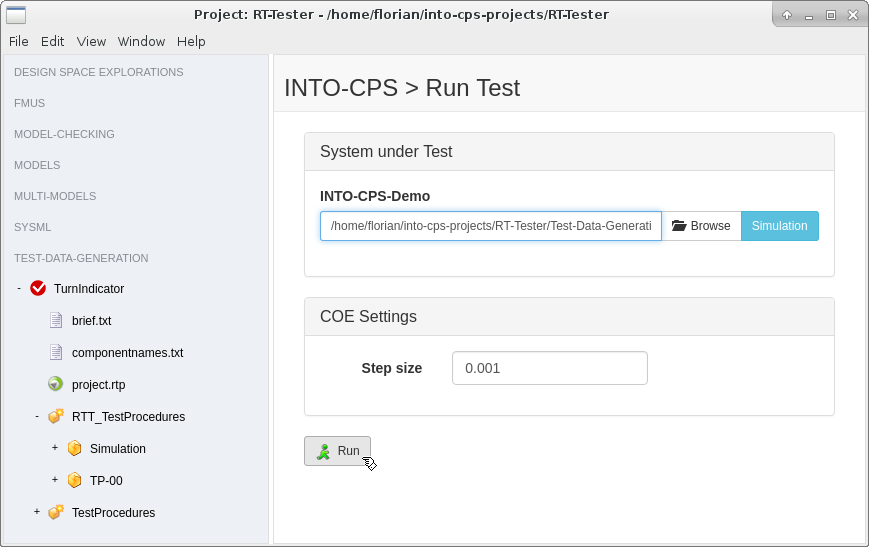
\includegraphics[width=\textwidth]{figures/VSI-TDG_Run-Test-Dialog}}
    \caption{Configuring a test.}
    \label{figure:INTO-CPS-App:Run-Test-Dialog}
\end{figure}
%
%
%

Every test execution yields as its result an
evaluation of test cases, \emph{i.\@e.\@}, each is associated with a verdict of PASS, FAIL, or
INCONCLUSIVE.\footnote{The verdict can also be NOT TESTED.  This means a
test case has been included in a test procedure, but a run that reaches it is still missing.}
The details are found in the test log files below the folder \path{testdata}.  See the RT-Tester user manual
\cite{VSI-rtt-man} for details. 

The file \path{testcase_tags.txt}
gives a condensed record of test case,
verdict, and point in a \path{*.log} file where a corresponding PASS, FAIL,
or---in case of INCONCLUSIVE---test case occurrence without assertion can be found.  The project-wide test-case verdict summary as well the requirement verdict summary
can be found in the folder \path{RTT_TestProcedures/verification}.
%
More details on the evaluation of test runs can be found in Deliverable D5.2a \cite{INTOCPSD5.2a}.
%
%
%
\subsection{Model Checking}\label{section:model:user-interface-integration}
This section describes how to use the INTO-CPS Application
as a front-end to the LTL model checker of RT-Tester RTT-MBT.
More details on the algorithms used and the syntax of
LTL formulas can be found in Deliverable D5.3c \cite{INTOCPSD5.3c}.

Once an INTO-CPS project has been created (see Section \ref{sub:projects}),
model checking functionality can be found
under the top-level activity \emph{Model Checking} in the project browser.
%
%\paragraph{Starting the License Management Process:}
Before getting started, the RT-Tester license management process must be launched.
%
To this end, right-click on \emph{Model Checking} and select \emph{Start RT-Tester License Dongle}
(see Figure \ref{figure:INTO-CPS-App:MC:Start-License-Dongle}).
%
%
%
\begin{figure}[ht]
    \centerline{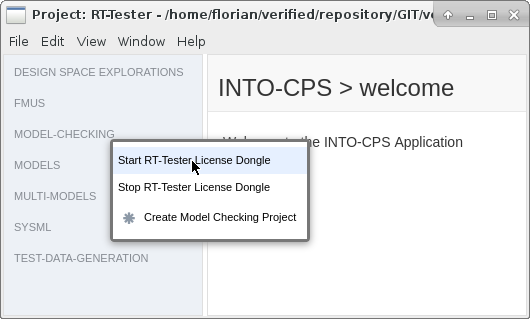
\includegraphics[width=0.7\textwidth]{figures/VSI-MC_Start-License-Dongle}}
    \caption{Starting the RT-Tester license dongle.}
    \label{figure:INTO-CPS-App:MC:Start-License-Dongle}
\end{figure}
%
%
%
Model checking projects are presented as sub-projects of INTO-CPS Application projects.
In order to add a new project,
%
%
%
\begin{enumerate}
\item  Right-click on the top-level activity \emph{Model Checking}
in the project browser and select \emph{Create Model Checking Project} (see
Figure \ref{figure:INTO-CPS-App:Create-MC-Project}).
%
\item  Provide a project name and the behavioural model that has been exported to XMI from Modelio (see \cref{sec:SysML:BehaviouralModelling}).
\end{enumerate}
%
%
%
\begin{figure}[ht]
    \centerline{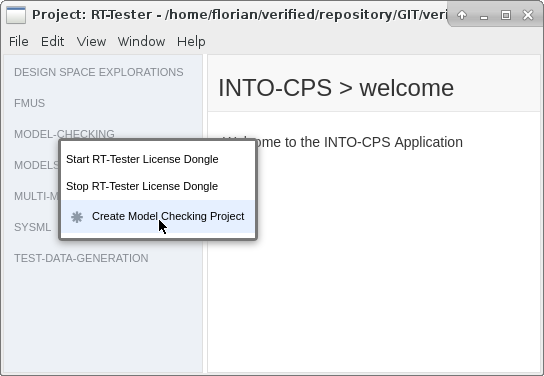
\includegraphics[width=0.7\textwidth]{figures/VSI-MC_Create-MC-Project}}
    \caption{Creating a model checking project.}
    \label{figure:INTO-CPS-App:Create-MC-Project}
\end{figure}
%
%
%
\begin{figure}[ht]
    \centerline{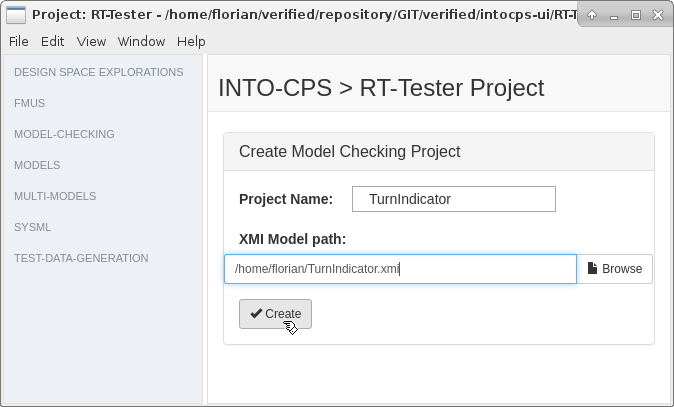
\includegraphics[width=0.8\textwidth]{figures/VSI-MC_Create-MC-Project-Dialog}}
    \caption{Specifying the model checking project.}
    \label{figure:INTO-CPS-App:Create-MC-Project-Dialog}
\end{figure}
\clearpage
%
%
%
After pressing \emph{Create}, a new node representing the model checking project is added to
the project browser.

%\paragraph{Adding, Editing and Checking LTL Queries:}
The next step is to add LTL queries to the project:
%
%
%
\begin{enumerate}
\item  Right click on the project and select \emph{Add LTL Query} (see Figure \ref{figure:INTO-CPS-App:Add-LTL}).
%
\item  Enter a name for the new query (see Figure \ref{figure:INTO-CPS-App:Add-LTL-Dialog}).
%
\item  To edit the LTL query, double click on the corresponding node in the project browser
(see Figure \ref{figure:INTO-CPS-App:Open-LTL}).  The LTL formula can then be edited in a text field.
In addition to all variables occurring in the model a special variable called \emph{\_stable} which is true \emph{iff} the system resides in a stable state is available.
This variable can be used to rule out spurious counter-examples involving transient states
that are immediately left in zero time.
Note that the editor supports
auto-completion for variable names and LTL operators (see
Figure \ref{figure:INTO-CPS-App:Edit-LTL-Completion}).
%
\item Specify a comma-separated list of requirements and select whether a
model checking result should be linked to either verify or violate these requirements
in the traceability database.
%
\item  Provide the upper bound for the bounded model checking query.
\end{enumerate}
%
%
%
\begin{figure}[ht]
    \centerline{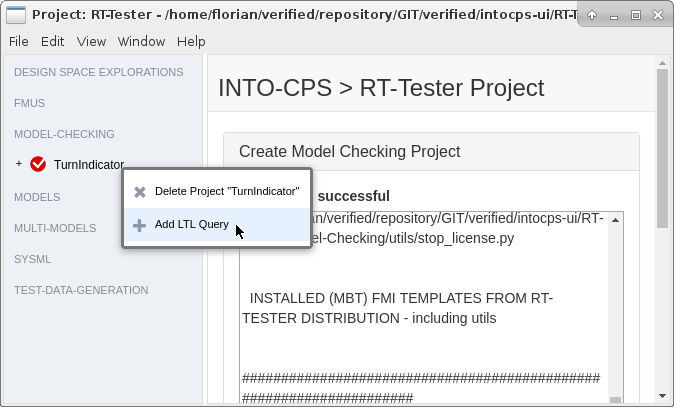
\includegraphics[scale=0.4]{figures/VSI-MC_Add-LTL}}
    \caption{Adding an LTL formula.}
    \label{figure:INTO-CPS-App:Add-LTL}
\end{figure}
%
%
%
\begin{figure}[ht]
    \centerline{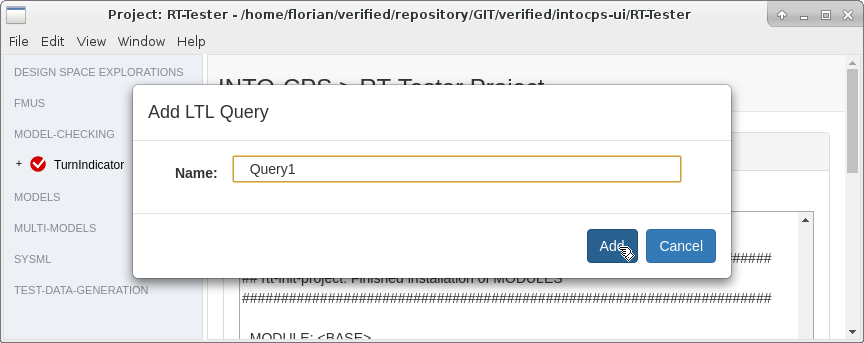
\includegraphics[scale=0.4]{figures/VSI-MC_Add-LTL-Dialog}}
    \caption{Naming the new LTL formula.}
    \label{figure:INTO-CPS-App:Add-LTL-Dialog}
\end{figure}
%
%
%
\begin{figure}[ht]
    \centerline{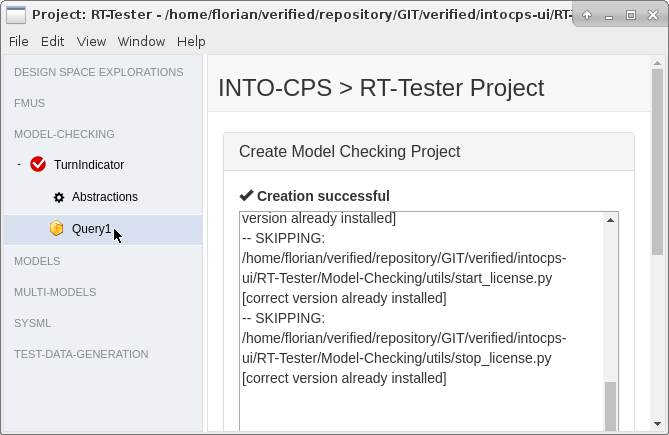
\includegraphics[scale=0.4]{figures/VSI-MC_Open-LTL}}
    \caption{Opening the LTL formula editor.}
    \label{figure:INTO-CPS-App:Open-LTL}
\end{figure}
%
%
%
\begin{figure}[ht]
    \centerline{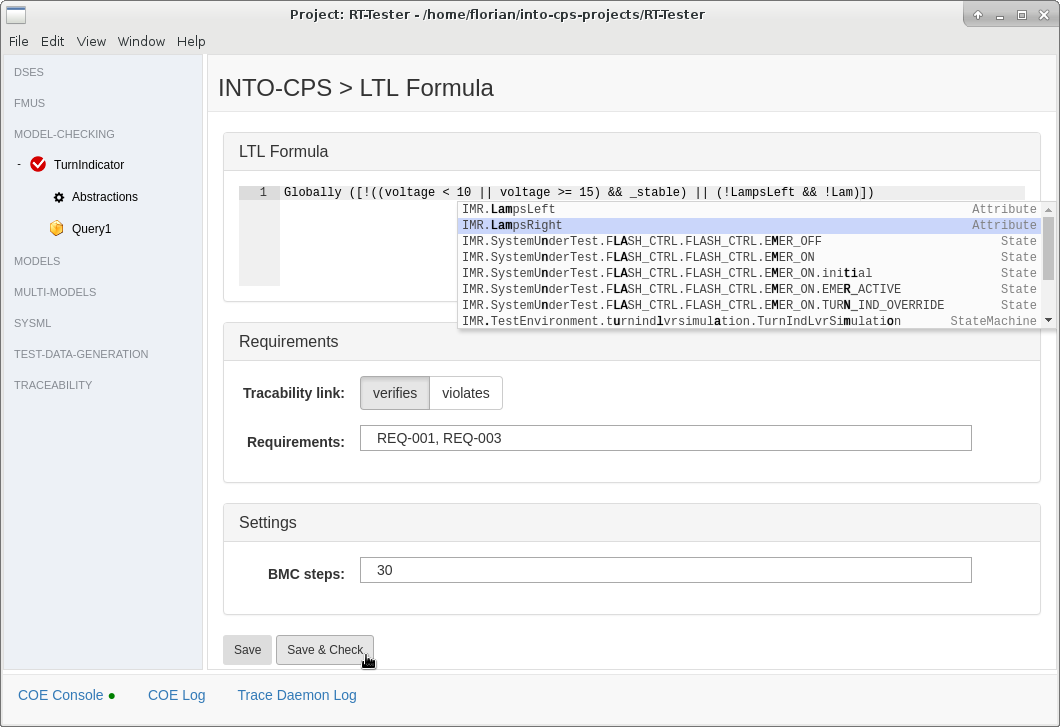
\includegraphics[width=\textwidth]{figures/VSI-MC_Edit-LTL-Completion}}
    \caption{LTL formula editor.}
    \label{figure:INTO-CPS-App:Edit-LTL-Completion}
\end{figure}
%
%
%
To check the query, press \emph{Save \& Check}.
After a while the tool either reports that the query holds within the specified number of steps or it prints a counterexample to demonstrate that the property does not hold --- as depicted in
Figure \ref{figure:INTO-CPS-App:Add-LTL-Checked}.
The user then has to manually inspect the model-checking result for spurious counter examples
that might have been introduced by abstractions that are too coarse.
Finally, if the user is satisfied with the result, the traceability information associated
with the result can be committed to the traceability database by pressing
\emph{Commit Traceability Data}.
%
%
%
\begin{figure}[ht]
    \centerline{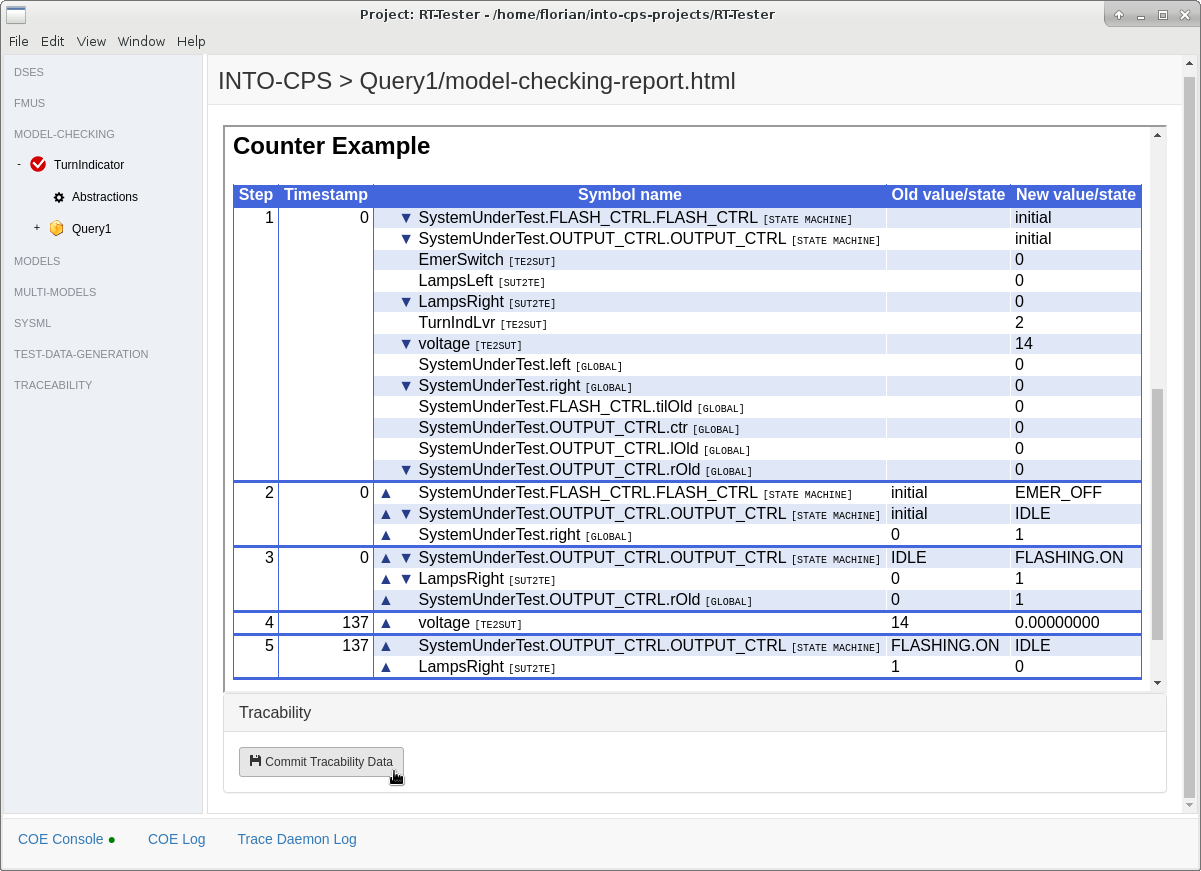
\includegraphics[scale=0.4]{figures/VSI-MC_Add-LTL-Checked}}
    \caption{Model checking result.}
    \label{figure:INTO-CPS-App:Add-LTL-Checked}
\end{figure}
%
%
%

It is possible to configure
abstractions\footnote{Information on abstractions and their associated configuration items can be found in Deliverable D5.2b \cite{INTOCPSD5.2b}.} for a particular model checking project.
%
To do so, double-click on
the corresponding \emph{Abstractions} node below that project in the project browser.
It is then possible to choose an abstraction method for each output variable of an
environment component along with making the associated setting. In
Figure \ref{figure:INTO-CPS-App:Configure-Abstractions-Dialog} the interval abstraction has
been selected for the output variable \texttt{voltage}. This abstraction has further been
configured to restrict the variable's value within the interval $[10,12]$. After pressing
\emph{Save}, this abstraction is applied to all model checking queries in the current
model checking project.
%
%
%
\begin{figure}[ht]
    \centerline{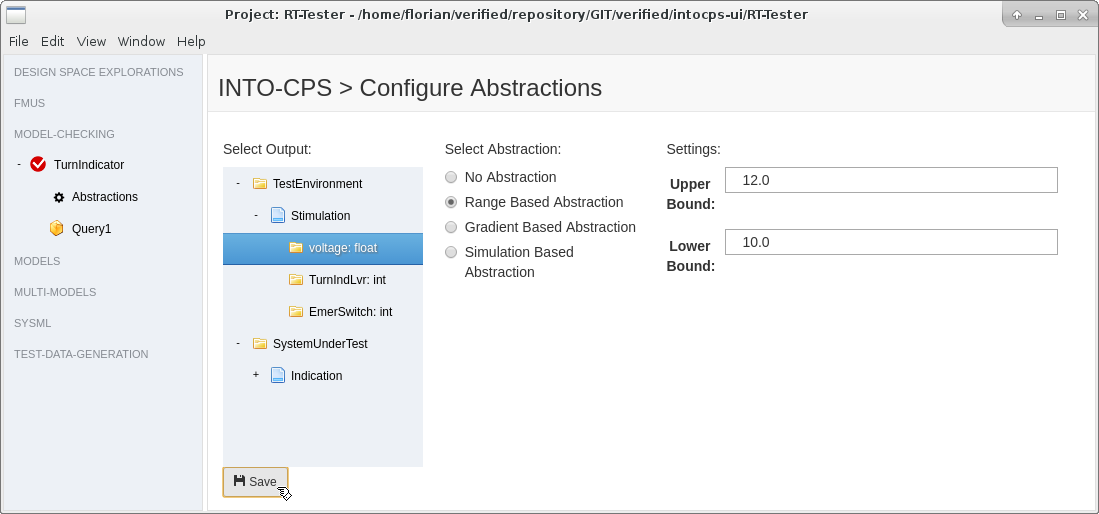
\includegraphics[width=\textwidth]{figures/VSI-MC_Configure-Abstractions-Dialog.png}}
    \caption{Configuring abstractions.}
    \label{figure:INTO-CPS-App:Configure-Abstractions-Dialog}
\end{figure}
%
%
%% ----------------------------------------------------------------------
%% $Revision: 6391 $
%% $Id: ta-modelling-guidelines.tex 6391 2017-06-08 14:13:27Z oliver.moeller@verified.de $
%% $URL: https://svn.nfit.au.dk/svn/iha_pgl-INTOCPS/WP4/D4_3a_User_Manual/sections/ta-modelling-guidelines.tex $
%% ----------------------------------------------------------------------
%% @TABLE OF CONTENTS:                 [TOCD: 15:26 08 Jun 2017]
%%
%% ----------------------------------------------------------------------
%% @SPELL: british                      Thu Jun  8 16:12:01 2017
%% ----------------------------------------------------------------------
\subsection{Modeling Guidelines (for TA and MC purposes)}\label{sec:modeling.guidelines.TA.MC}
When creating a model for test automation (TA) or model checking (MC), it is
important to keep in mind that it will be input to a {\em solver} that
explores the state space of the model. 
It is not helpful to have a very precise state machine model which the solver
cannot handle.\footnote{\emph{I.\@e.\@}, resources on time, memory or user patience will
  be depleted before completion of the ``solving'' task.} 

A {\em ``good''} model tries to find a balance between precision and solver
time, \emph{i.\@e.\@}, it aims to represent all important logical aspects (that may
contain design errors,) but abstract away from details where the
implementation can be trusted to handle data correctly.
%
This section contains some guidelines on how to avoid common modelling pitfalls.
%
\paragraph{(G.1) Model independent parts as separate machines.}
When you can think of two parts of the system as individual entities, then
you should have one state machine for each part. This is much easier to
maintain than a state machine that ``merges'' two (or more) behaviours.
%
\paragraph{(G.2) Reset auxiliary variables.}
If you use ``auxiliary'' variables in your model (\emph{e.\@g.\@} to remember some
situation) then they should have a limited lifetime where they can be of
relevance.  Reset them (to ``0'') when they have fulfilled their purpose. This modelling
trick will not influence the relevant behaviour of your model, but make the solver's task easier.
%
\paragraph{(G.3) Keep the diameter of state machines small (if possible).}
The number of steps that are necessary to reach a certain situation can be a
serious limitation in finding solutions.  If your state machine includes long sequences of transitions that need to be
taken in order to reach a certain situation, consider simplifying it by
\begin{itemize}
\item breaking this state machine down into several state machines
\item ``merging'' several similar states along this path into a single, more
  abstract state (\emph{i.\@e.\@} make your model less precise)
\end{itemize}
%
\paragraph{(G.4) Use abstractions whenever specific (payload) data is of no interest.}
If the logical state depends on input data, try to model this as simply as
possible. Consider omitting data sanitation steps (like plausibility checks,
interpolation of values, data sanitation) that may exist in your specific
system but only serve as countermeasures to unreliable sensor inputs. In the
modelling world, inputs are always ``perfect'' and ``reliable''.
{\bf Example}: When modelling a protocol, avoid modelling the payload. Also, do not put payload and addressing (housekeeping) information in the
same variable.
%
\paragraph{(G.5) Try to think of ``logical states'' rather than of ``data driven states''.}
Variables can be used to ``encode'' the states of your system. Try to find a
balance where state machine states actually represent ``logical states'' (that
are distinguished by their behaviour). This will make the guard conditions
smaller and more maintainable.
%
\paragraph{(G.6) Keep a list of modelling parameters.}
Keep an overview on what immutable ``parameters'' your modelling depends on,
\emph{i.\@e.\@}, what values they have and where they are used.
This will make it easier to revise your model consistently when required.
%
\paragraph{(G.7) Dare to approximate complex values.}
In particular {\em continuous flows} may need to be broken down into manageable
components.
{\bf Example}: A physical accumulator can be approximated by a scalar value. 
Using a (scaled) integer instead of a floating-point number may be good enough and make the
task of the solver much easier.
%
\paragraph{(G.8) Dare to approximate complex behaviour.}
A common modelling mistake is to ``model as precise as possible''. 
In particular, capturing continuous states can be very expensive (in terms of
state space).  Whenever possible, you should consider simplifying things, even if this
means sacrificing precision. Remember that testing aims to find ``logical
errors'' and not to ``represent the most precise approximation of the system''.
{\bf Example}: When modelling a water tank with (continuous) in-flow and state
change, it may suffice to create a ``coarse'' model of it which changes state
only once per second, based in input value, water level, and maximal output
capacity. 
%
\paragraph{(G.9) Start with small versions of your system.}
Do not start modelling with a full-blown version of a complete system. Rather
start with one relevant component, say, one controller and explore testing a
small system
before moving to ``many controllers, many other components''.
%% -------------------------------------------------------------------------